\subsubsection{Datenbankzugriff}                   
Für den Datenzugriff auf die Datenbank wurden zu jeder Collection Service-Module erstellt, die entsprechenden Zugriff gewähren. Dafür wurden innerhalb der Service-Modulen die benötigten Zugriffsfunktionen implementiert.

\begin{figure}[h]
\centering
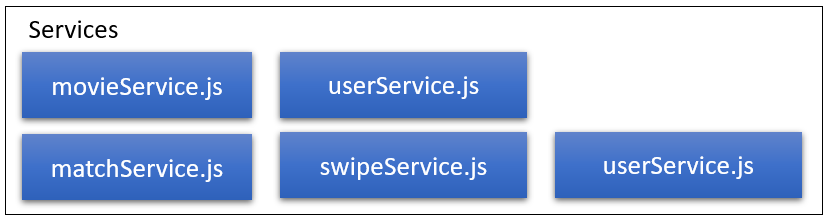
\includegraphics[width=8cm]{images/serviceStruktur.PNG}
\caption{Node.js Server - Services Struktur}
\end{figure}

\paragraph{Movie Service}
Nachfolgend werden die Funktionen des Moduls movieService.js beschrieben.

\subparagraph{FindMoviesExcept}
Der Funktion

\begin{lstlisting}[caption=movieService.js - FindMoviesExcept, label=lst:findmoviesexcept]
const Movie = require('../database/models/movie')

async function FindMoviesExcept(excludedMovies, amount) {
    var movies;

    try{  movies = await Movie.find({ id: { $nin: excludedMovies }}).limit(amount); } //https://docs.mongodb.com/manual/reference/operator/query/nin/      }
    catch(err){  throw err;}

    return movies;
}

module.exports.FindMoviesExcept = FindMoviesExcept;
\end{lstlisting}

\paragraph{User Service}
Nachfolgend werden die Funktionen des Moduls userService.js beschrieben.

\subparagraph{CreateUser}
Die

\begin{lstlisting}[caption=TODO, label=lst:TODO]
xx
\end{lstlisting}

\subparagraph{CheckExistence}
Die

\begin{lstlisting}[caption=TODO, label=lst:TODO]
xx
\end{lstlisting}

\subparagraph{GetCityFromUser}
Die

\begin{lstlisting}[caption=TODO, label=lst:TODO]
xx
\end{lstlisting}

\subparagraph{ChangeCityFromUser}
Die

\begin{lstlisting}[caption=TODO, label=lst:TODO]
xx
\end{lstlisting}

\subparagraph{ChangeGenderWantedFromUser}
Die

\begin{lstlisting}[caption=TODO, label=lst:TODO]
xx
\end{lstlisting}

\subparagraph{ChangeGenderFromUser}
Die

\begin{lstlisting}[caption=TODO, label=lst:TODO]
xx
\end{lstlisting}

\subparagraph{GetInfoFromUser}
Die

\begin{lstlisting}[caption=TODO, label=lst:TODO]
xx
\end{lstlisting}

\paragraph{Match Service}
Nachfolgend werden die Funktionen des Moduls 
matchService.js beschrieben.

\subparagraph{CreateUserMatchDocument}
Die

\begin{lstlisting}[caption=TODO, label=lst:TODO]
xx
\end{lstlisting}

\subparagraph{CheckMatch}
Die

\begin{lstlisting}[caption=TODO, label=lst:TODO]
xx
\end{lstlisting}

\subparagraph{AddNormalMatchToUser}
Die

\begin{lstlisting}[caption=TODO, label=lst:TODO]
xx
\end{lstlisting}

\subparagraph{AddSuperMatchToUser}
Die

\begin{lstlisting}[caption=TODO, label=lst:TODO]
xx
\end{lstlisting}

\subparagraph{GetMatches}
Die

\begin{lstlisting}[caption=TODO, label=lst:TODO]
xx
\end{lstlisting}

\subparagraph{SuperMatchMarkAsRemoved}
Die

\begin{lstlisting}[caption=TODO, label=lst:TODO]
xx
\end{lstlisting}

\subparagraph{NormalMatchMarkAsRemoved}
Die

\begin{lstlisting}[caption=TODO, label=lst:TODO]
xx
\end{lstlisting}

\subparagraph{MatchesReceived}
Die

\begin{lstlisting}[caption=TODO, label=lst:TODO]
xx
\end{lstlisting}

\paragraph{Swipe Service}
Nachfolgend werden die Funktionen des Moduls 
swipeService.js beschrieben.

\subparagraph{CreateUserSwipeDocument}
Die

\begin{lstlisting}[caption=TODO, label=lst:TODO]
xx
\end{lstlisting}

\subparagraph{AddSwipe}
Die

\begin{lstlisting}[caption=TODO, label=lst:TODO]
xx
\end{lstlisting}

\subparagraph{RequestSwipes}
Die

\begin{lstlisting}[caption=TODO, label=lst:TODO]
xx
\end{lstlisting}

\subparagraph{RequestSuperlikeSwipes}
Die

\begin{lstlisting}[caption=TODO, label=lst:TODO]
xx
\end{lstlisting}

\subparagraph{FindAllSwipedMoviesByUserID}
Die

\begin{lstlisting}[caption=TODO, label=lst:TODO]
xx
\end{lstlisting}
